\documentclass[11pt]{article}
\usepackage{../../latex/stat4ml_style}

\title{Chapter 7: Bayesian Estimation \\ \large Part I --- Statistics Foundation for ML}
\author{Omid Safarzadeh}
\date{}

\begin{document}
\maketitle

\begin{abstract}
\noindent
Maximum likelihood (Chapter 6) treats the parameter as a fixed unknown and
asks which value best explains the data. The Bayesian view instead treats
the parameter as a random quantity with a distribution: you start with a
\emph{prior}, see data, and update to a \emph{posterior} by Bayes' rule.
This chapter builds that update, shows the conjugate families where it stays
a one-line formula, and closes by connecting the two philosophies --- with
enough data the posterior concentrates into the same normal the
maximum-likelihood estimator obeys, so Bayesian and frequentist answers meet.
\end{abstract}

\tableofcontents

% ======================================================================
\section{Prior, likelihood, posterior}
% ======================================================================

Write $\pi(\theta)$ for the \keyterm{prior} --- what you believe about the
parameter before seeing data --- and $L(x \mid \theta)$ for the likelihood.
Bayes' rule combines them into the \keyterm{posterior}.

\begin{definition}[Posterior]
\[
  \pi(\theta \mid x) = \frac{L(x\mid\theta)\,\pi(\theta)}{\int L(x\mid\theta')\,\pi(\theta')\,d\theta'}
  \;\propto\; L(x\mid\theta)\,\pi(\theta).
\]
The denominator is a constant in $\theta$, so the shape of the posterior is
just likelihood times prior; it is normalised at the end to integrate to one.
\end{definition}

From the posterior come the usual summaries: the \keyterm{posterior mean}
$E[\theta\mid x]$, the \keyterm{maximum a posteriori} (MAP) estimate
$\arg\max_\theta \pi(\theta\mid x)$, and a \keyterm{credible interval}, an
interval holding, say, $95\%$ of the posterior probability.

The cleanest case is when prior and posterior belong to the same family ---
the prior is \keyterm{conjugate} to the likelihood --- so updating only
changes the parameters. The headline example is the Beta prior with
Bernoulli/Binomial data.

\begin{theorem}[Beta--Binomial conjugacy]
With prior $\theta \sim \mathrm{Beta}(\alpha,\beta)$ and $k$ successes in
$n$ independent trials, the posterior is
$\theta \mid x \sim \mathrm{Beta}(\alpha + k,\; \beta + n - k)$.
\end{theorem}

Its posterior mean, $\frac{\alpha+k}{\alpha+\beta+n}$, is a blend of the
prior and the data that slides toward the sample proportion $k/n$ as $n$
grows. Conjugacy makes several models one-liners:

\begin{lstlisting}[language=Python]
def beta_binomial(alpha, beta, k, n):             # Beta prior, Binomial data
    return (alpha + k, beta + n - k)              # -> Beta(.,.)

def gamma_poisson(a, b, total, n):                # Gamma(a,b) prior, Poisson data
    return (a + total, b + n)                     # -> Gamma(shape, rate)

def normal_normal(mu0, tau2, xbar, sigma2, n):    # Normal prior, known variance
    prec = 1 / tau2 + n / sigma2
    mean = (mu0 / tau2 + n * xbar / sigma2) / prec
    return (mean, 1 / prec)                       # -> Normal(mean, variance)

print(beta_binomial(1, 1, 8, 10))                 # (9, 3)
print(gamma_poisson(2, 1, 30, 10))                # (32, 11)
print(normal_normal(0, 1, 2.0, 1.0, 10))          # (1.818..., 0.0909...)
\end{lstlisting}

\noindent Each line is a complete inference: feed the prior parameters and
the data, read off the posterior. The figure shows the Beta--Binomial case
as flips accumulate --- a flat prior sharpening into a tight posterior around
the true $p$.

\begin{figure}[h]
  \centering
  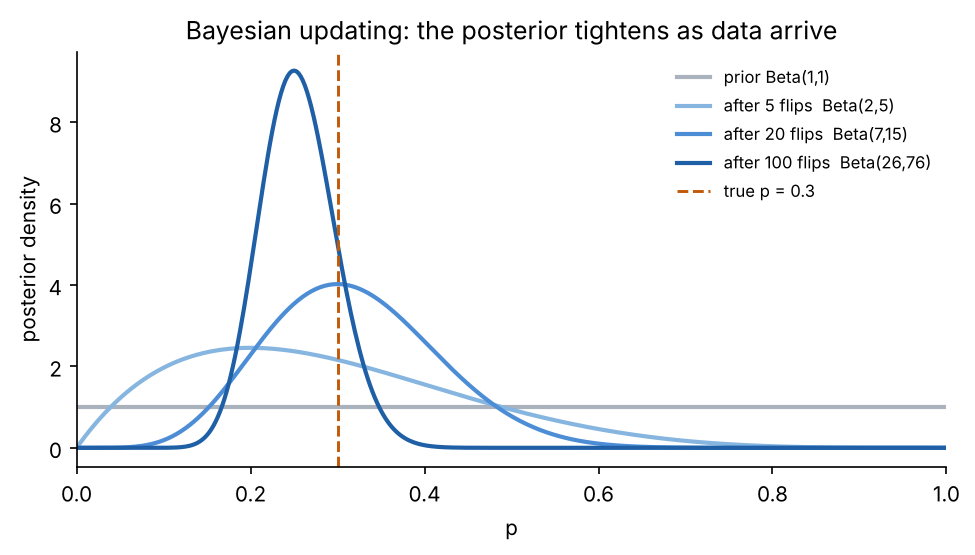
\includegraphics[width=0.86\linewidth]{figures/posterior_update.png}
\end{figure}

% ======================================================================
\section{Why the updates work}
% ======================================================================

Both conjugate formulas above come straight from ``posterior $\propto$
likelihood $\times$ prior,'' with the algebra being a matter of collecting
exponents.

\begin{theorem}[Proof of Beta--Binomial]
The Binomial likelihood in $\theta$ is $\theta^{k}(1-\theta)^{n-k}$ and the
Beta prior is $\propto \theta^{\alpha-1}(1-\theta)^{\beta-1}$. Multiplying,
\[
  \pi(\theta\mid x) \;\propto\;
  \theta^{k}(1-\theta)^{n-k}\,\theta^{\alpha-1}(1-\theta)^{\beta-1}
  = \theta^{(\alpha+k)-1}(1-\theta)^{(\beta+n-k)-1},
\]
which is the kernel of $\mathrm{Beta}(\alpha+k,\,\beta+n-k)$.
\end{theorem}

The Normal case is just as mechanical, and the answer is worth stating in
words: posterior precisions add, and the posterior mean is a
precision-weighted average.

\begin{theorem}[Normal--Normal, known variance]
With prior $\theta \sim N(\mu_0,\tau^2)$ and $n$ observations of mean
$\bar x$ from $N(\theta,\sigma^2)$, the posterior is normal with
\[
  \text{precision } \frac{1}{\tau^2} + \frac{n}{\sigma^2},
  \qquad
  \text{mean } \frac{\mu_0/\tau^2 + n\bar x/\sigma^2}{1/\tau^2 + n/\sigma^2}.
\]
\end{theorem}
\begin{proof}[Sketch]
Both prior and likelihood are exponentials of quadratics in $\theta$. Adding
the exponents gives another quadratic, $-\tfrac12\big(\tfrac{1}{\tau^2} +
\tfrac{n}{\sigma^2}\big)\theta^2 + \big(\tfrac{\mu_0}{\tau^2} +
\tfrac{n\bar x}{\sigma^2}\big)\theta + \text{const}$. Completing the square
reads off a normal whose precision is the coefficient of $-\tfrac12\theta^2$
and whose mean is the stated ratio.
\end{proof}

\noindent Notice what the weights do: a tight prior (small $\tau^2$) or a lot
of data (large $n$) pulls the posterior mean toward that side. The prior
behaves like $1/\tau^2$ worth of ``pseudo-observations.''

% ======================================================================
\section{Priors, prediction, and the link to maximum likelihood}
% ======================================================================

Two estimates summarise a posterior, and they usually differ: the
\keyterm{posterior mean} $E[\theta\mid x]$ minimises expected squared error,
while the \keyterm{MAP} estimate $\arg\max\pi(\theta\mid x)$ is the posterior
mode. For a symmetric posterior they coincide; for a skewed one they do not.
MAP with a flat prior is just maximum likelihood, which is the first hint
that the two frameworks are close.

To predict a new observation one averages the likelihood over the posterior
rather than plugging in a point estimate --- the \keyterm{posterior
predictive}
\[
  p(x_{\text{new}}\mid x) = \int p(x_{\text{new}}\mid\theta)\,\pi(\theta\mid x)\,d\theta,
\]
which carries the parameter uncertainty forward instead of pretending
$\theta$ is known exactly.

Where does the prior come from? One principled default is the
\keyterm{Jeffreys prior} $\pi(\theta)\propto\sqrt{I(\theta)}$, built from the
Fisher information of Chapter 6 so that it is invariant to how the parameter
is written. And whatever the prior, its influence fades: as data accumulate,
the likelihood dominates and the posterior forgets where it started. The
precise statement is the bridge back to Chapter 6.

\begin{theorem}[Bernstein--von Mises, informal]
Under regularity, for large $n$ the posterior is approximately
\[
  \theta \mid x \;\approx\; N\!\big(\hat\theta_{\text{MLE}},\; I_n(\theta)^{-1}\big),
\]
centred at the maximum-likelihood estimate with variance the inverse Fisher
information.
\end{theorem}

\noindent So in large samples a Bayesian credible interval and a frequentist
confidence interval very nearly coincide, and the choice of prior stops
mattering. The approximation itself --- fit a normal at the posterior mode
using the local curvature --- is the \keyterm{Laplace approximation}, the
workhorse behind practical Bayesian deep learning in Part III.

\begin{summarybox}
Bayesian estimation updates a prior to a posterior by
$\pi(\theta\mid x)\propto L(x\mid\theta)\pi(\theta)$. Conjugate families keep
this a formula: Beta--Binomial gives $\mathrm{Beta}(\alpha+k,\beta+n-k)$,
Normal--Normal adds precisions and takes a precision-weighted mean. Summaries
are the posterior mean, the MAP estimate, and credible intervals; prediction
integrates over the posterior. As $n\to\infty$ the posterior concentrates to
$N(\hat\theta_{\text{MLE}}, I_n^{-1})$ (Bernstein--von Mises), so the Bayesian
and maximum-likelihood answers meet.
\end{summarybox}

\end{document}
